\documentclass{article}

\usepackage{fancyhdr}
\usepackage{extramarks}
\usepackage{amsmath}
\usepackage{amsthm}
\usepackage{amsfonts}
\usepackage{tikz}
\usepackage[plain]{algorithm}
\usepackage{algpseudocode}
\usepackage{enumerate}
\usepackage{mathrsfs}
\usepackage{bm}
\usepackage{amssymb}
\usepackage{tikz}  
\usepackage{optidef}
\usepackage{pdfpages}
\usetikzlibrary{arrows.meta}
\usetikzlibrary{automata,positioning}

%
% Basic Document Settings
%  

\topmargin=-0.45in
\evensidemargin=0in
\oddsidemargin=0in
\textwidth=6.5in
\textheight=9.0in
\headsep=0.25in

\linespread{1.1}

\pagestyle{fancy}
\lhead{\hmwkAuthorName}
\rhead{\hmwkClass\ (\hmwkClassInstructor): \hmwkTitle}
\cfoot{\thepage}

\renewcommand\headrulewidth{0.4pt}
\renewcommand\footrulewidth{0.4pt}

\setlength\parindent{2em}

%
% Create Problem Sections
%


% \setcounter{secnumdepth}{0}
% \newcounter{partCounter}
% \newcounter{homeworkProblemCounter}
% \setcounter{homeworkProblemCounter}{1}


\newcommand{\hmwkTitle}{Homework III}
\newcommand{\hmwkDueDate}{Nov 16th, 2022}
\newcommand{\hmwkClass}{Introduction to Machine Learing}
\newcommand{\hmwkClassInstructor}{Professor Ziping Zhao}
\newcommand{\hmwkAuthorName}{Bingnan Li}
\newcommand{\hmwkAuthorID}{2020533092}

%
% Title Page
%

\title{
    \vspace{2in}
    \textmd{\textbf{\hmwkClass:\\ \hmwkTitle}}\\
    \normalsize\vspace{0.1in}\small{Due\ on\ \hmwkDueDate\ at 11:59pm}\\
    \vspace{0.1in}\large{\textit{\hmwkClassInstructor}}
    \vspace{3in}
}

\author{\textbf{\hmwkAuthorName}\\ \hmwkAuthorID}
\date{}

% \renewcommand{\part}[1]{\textbf{\large Part \Alph{partCounter}}\stepcounter{partCounter}\\}

%
% Various Helper Commands
%

% Useful for algorithms
\newcommand{\alg}[1]{\textsc{\bfseries \footnotesize #1}}

% For derivatives
\newcommand{\deriv}[1]{\frac{\mathrm{d}}{\mathrm{d}x} (#1)}

% For partial derivatives
\newcommand{\pderiv}[2]{\frac{\partial}{\partial #1} (#2)}

% Integral dx
\newcommand{\dx}{\mathrm{d}x}

% Alias for the Solution section header
\newcommand{\solution}{\textbf{\large Solution}}

% Probability commands: Expectation, Variance, Covariance, Bias
\newcommand{\E}{\mathbb{E}}
\newcommand{\Var}{\mathrm{Var}}
\newcommand{\Cov}{\mathrm{Cov}}
\newcommand{\Bias}{\mathrm{Bias}}
\renewcommand{\b}[1]{\bm{#1}}
\newcommand{\PARTIAL}[2]{\frac{\partial #1}{\partial #2}}
\begin{document}

\maketitle
\pagebreak

\begin{enumerate}
    \setlength\parindent{2em}
    \item [1.] [SVM]
    \begin{enumerate}
        \item [(a)] Hard-margin SVM
        \begin{enumerate}
            \setlength\parindent{2em}
            \item [(i)] Lagrangian function and dual representation:\newline
            {\bf Solution:}
            \par By introducing Lagrangian multipliers $\{\alpha_i\}$, we have the Lagrangian function $\mathcal{L}$
            \begin{align*}
                \mathcal{L}(\b{w},w_0,\{\alpha_i\}) &= \frac{1}{2}||\b{w}||_2^2 - \sum_{i=1}^N\alpha_i\left[r^i(\b{w}^T\b{x}^i+w_0)-1\right]\\
                &= \frac{1}{2} \b{w}^T\b{w} - \b{w}^T\sum_{i=1}^N\alpha_i r^i\b{x}^i-w_0\sum_{i=1}^N\alpha_ir^i+\sum_{i=1}^N\alpha_i
            \end{align*}
            Then by zero gradient theorem, we have 
            \begin{align}
                \frac{\partial \mathcal{L}}{\partial \b{w}} &=\b{w}-\sum_{i=1}^N\alpha_ir^i\b{x}^i=0 \Rightarrow\b{w}=\sum_{i=1}^N\alpha_ir^i\b{x}^i\\
                \frac{\partial \mathcal{L}}{\partial w_0} &=-\sum_{i=1}^N\alpha_ir^i=0 \Rightarrow \sum_{i=1}^N\alpha_ir^i=0
            \end{align}
            By substituting $\b{w}$ and $\sum_{i=1}^N\alpha_ir^i$ with equation (1) and (2), we have 
            \begin{align*}
                G(\{\alpha_i\})=\sum_{i=1}^N\alpha_i-\frac{1}{2}\sum_{i=1}^N\sum_{j=1}^N\alpha_i\alpha_jr^ir^j(\b{x^i})^T\b{x^j}
            \end{align*}
            Thus, the dual representation is as following:
            \begin{align*}
                {maximize}_{\{\alpha_i\}} &\sum_{i=1}^N\alpha_i-\frac{1}{2}\sum_{i=1}^N\sum_{j=1}^N\alpha_i\alpha_jr^ir^j(\b{x^i})^T\b{x^j}\\
                subject\ to\ &\sum_{i=1}^N\alpha_ir^i=0\\
                &\alpha_i\geq 0,\forall i
            \end{align*}
            \item [(ii)] Show that $\frac{1}{\gamma_{max}^2}=\sum_{i=1}^N\alpha_i$.\newline
            {\bf Proof:}
            \par Define 
            \[\b{\alpha}=\begin{bmatrix}
                \alpha_1\\
                \vdots\\
                \alpha_N
            \end{bmatrix}\quad
            \b{r} = \begin{bmatrix}
                r^1\\
                \vdots\\
                r^N
            \end{bmatrix} \]
            and symmetric matrix $\b{H}$ with $h_{ij}=r^ir^j(x^i)^Tx^j$.
            Then the dual representation of maximum margin problem can be rewritten as following
            \begin{align*}
                maximize_{\b{\alpha}}\ &\b{\alpha^T 1}-\frac{1}{2}\b{\alpha^T H \alpha}\\
                subject\ to\ &\b{\alpha^T r} = 0\\
                &\b{\alpha}\geq \b{0}
            \end{align*}
            Then the Lagrangian function is 
            \begin{align*}
                \mathcal{L}(\b{\alpha}, \b{\lambda}, v) = \frac{1}{2}\b{\alpha^TH\alpha}-\b{\alpha^T 1} + \b{\lambda^T \alpha} + v\b{\alpha^Tr}
            \end{align*}
            and the corresponding KKT conditions are
            \begin{align*}
                \left\{\begin{aligned}
                    &\PARTIAL{\mathcal{L}}{\b{\alpha}} = \b{H\alpha}-\b{1}-\b{\lambda}+v\b{r}=0\\
                    &\b{\alpha^T r} = 0, \b{\alpha}\geq \b{0}\\
                    &\b{\lambda} \geq 0\\
                    &\b{\alpha^T \lambda} = 0
                \end{aligned}\right.
            \end{align*}
            Thus, we have 
            \begin{align*}
                \mathcal{L} &= \frac{1}{2}\b{\alpha^T}(\b{1+\lambda}-v\b{r})-\b{\alpha^T 1}\\
                &=\frac{1}{2}\b{\alpha^T 1}-\b{\alpha^T 1}\\
                &=-\frac{1}{2}\b{\alpha^T 1}=-\frac{1}{2}\sum_{i=1}^N\alpha_i
            \end{align*}
            Which means the constraint minimum value of $\frac{1}{2}\b{\alpha^T H\alpha}-\b{\alpha^T 1}$ is $-\frac{1}{2}\sum_{i=1}^N\alpha_i$, then the constraint maximum value of $-\frac{1}{2}\b{\alpha^T H\alpha}+\b{\alpha^T 1}$ is $\frac{1}{2}\sum_{i=1}^N\alpha_i$. Moreover, the constraint minimum value of $\frac{1}{2}||\b{w}||_2^2$ is also $\frac{1}{2}\sum_{i=1}^N\alpha_i$.
            \par Thus, we have 
            \[||\b{w}||_{min}^2=\frac{1}{\gamma^2_{max}}=\sum_{i=1}^N\alpha_i\]
        \end{enumerate}
        \item [(b)]Soft-margin SVM\newline
        {\bf Proof:}
        \par The primal problem of soft margin SVM problem is as following:
        \begin{align*}
            minimize_{\b{w},w_0,\{\xi_t\}}\quad & \frac{1}{2}||\b{w}||^2+C\sum_{i=1}^N \xi_i\\
            subject\ to\quad & r^if(\b{x})\geq 1-\xi_i,\ \forall i\\
            & \xi_i\geq 0,\ \forall i
        \end{align*}
        and KKT conditions are
        \begin{align*}
            \left\{\begin{aligned}
                &\b{w}-\sum_{i=1}^N\alpha_i(r^ix^i)=0\\
                &\sum_{i=1}^N\alpha^ir^i=0\\
                &\mu_i=C-\alpha_i\\
                &\alpha^i\geq 0, \mu_i\geq 0\\
                &\alpha_i(r^if(\b{x})-1+\xi_i)=0,\mu_i\xi_i=0\\
                &r^if(x)-1+\xi_i\geq 0,\xi_i\geq 0
            \end{aligned}\right.
        \end{align*}
        If $\alpha_i=0$, we have 
        \begin{align*}
            \mu_i &= C-\alpha_i = C\\
            \mu_i\xi_i&=0\Rightarrow\xi_i=0\\
            \alpha_i(r^if(\b{x})-1+\xi_i)&=0, r^if(\b{x})-1+\xi_i \geq 0 \Rightarrow r^if(\b{x})-1+\xi_i\geq 0\\
            &\Rightarrow r^if(\b{x})\geq 1-\xi_i = 1
        \end{align*}

        If $0<\alpha_i<C$, we have 
        \begin{align*}
            \mu_i &= C-\alpha_i \neq 0\\
            \mu_i\xi_i &= 0\Rightarrow\xi_i=0\\
            \alpha_i(r^if(\b{x})-1+\xi_i)=0&\Rightarrow r^if(\b{x})-1= 0\\
            &\Rightarrow r^if(\b{x})= 1 
        \end{align*} 
        If $\alpha=C$, we have
        \begin{align*}
            \mu_i &= C-\alpha_i = 0\\
            \mu_i\xi_i &= 0, \xi_i\geq 0\Rightarrow\xi_i\geq 0\\
            \alpha_i(r^if(\b{x})-1+\xi_i)=0&\Rightarrow r^if(\b{x})=1-\xi_i\leq 1
        \end{align*}
    \end{enumerate}
    \item [2.] [SVM]
    \begin{enumerate}
        \item [(a)] Dual problem of SVR\newline
        {\bf Solution:}
        \par In order to convert SVR into dual QP problem, we introduce slack variables $\xi_i^+$ and $\xi_i^-$ and the primal problem is as following
        \begin{align*}
            minimize_{\b{w},\{\xi_i^+\},\{\xi_i^-\}}\quad & \frac{1}{2}||\b{w}||^2+C\sum_{i=1}^N(\xi_i^++\xi_i^-)\\
            subject\ to\quad & r^i-\b{w}^T\b{x}^i\leq \epsilon+\xi_i^+,\quad\forall i\\
            & \b{w}^T\b{x}^i-r^i\leq \epsilon+\xi_i^-,\quad\forall i\\
            & \xi_i^+,\xi_i^-\geq 0,\quad\forall i
        \end{align*}
        and the Lagrangian function is 
        \begin{align*}
            &\mathcal{L}(\b{w},\{\xi_i^+\},\{\xi_i^-\},\{\alpha_i^+\},\{\alpha_i^-\},\{\mu_i^+\},\{\mu_i^-\})\\
            &= \frac{1}{2}||\b{w}||^2+C\sum_{i=1}^N(\xi_i^++\xi_i^-)-\sum_{i=1}^N\alpha_i^+[\epsilon+\xi_i^+-r^i+\b{w}^T\b{x}^i]
            -\sum_{i=1}^N\alpha_i^-[\epsilon+\xi_i^-+r^i-\b{w}^T\b{x}^i]\\ &\quad-\sum_{i=1}^N(\mu_i^+\xi_i^++\mu_i^-\xi_i^-)
        \end{align*}
        By setting the gradient of $\mathcal{L}$ to 0, we have 
        \begin{align}
            \frac{\partial \mathcal{L}}{\partial \b{w}} &= \b{w}-\sum_{i=1}^N(\alpha_i^+-\alpha_i^-)\b{x}^i=\b{0}\\
            \PARTIAL{\mathcal{L}}{\xi_i^+} &= C-\alpha_i^+-\mu_i^+=0\\
            \PARTIAL{\mathcal{L}}{\xi_i^-} &= C-\alpha_i^--\mu_i^-=0+
        \end{align}
        Then, substitute $\b{w}, C$ with equation (3), (4) and (5), we have 
        \begin{align*}
            &G(\{\alpha_i^+\},\{\alpha_i^-\})\\
            &=-\frac{1}{2}\sum_{i=1}^N\sum_{j=1}^N(\alpha_i^+-\alpha_i^-)(\alpha_j^+-\alpha_j^-)(\b{x}^i)^T\b{x}^j-\epsilon\sum_{i=1}^N(\alpha_i^++\alpha_i^-)+\sum_{i=1}^N r^t(\alpha_i^+-\alpha_i^-)
        \end{align*}
        Thus, the dual problem is 
        \begin{align*}
            maximize_{\{\alpha_i^+\},\{\alpha_i^-\}}\qquad &-\frac{1}{2}\sum_{i=1}^N\sum_{j=1}^N(\alpha_i^+-\alpha_i^-)(\alpha_j^+-\alpha_j^-)(\b{x}^i)^T\b{x}^j\\
            &-\epsilon\sum_{i=1}^N(\alpha_i^++\alpha_i^-)+\sum_{i=1}^N r^t(\alpha_i^+-\alpha_i^-)\\
            subject\ to\qquad & 0\leq\alpha_i^+\leq C,\ \forall i\\
            & 0\leq \alpha_i^-\leq C,\ \forall i
        \end{align*}
        \item [(b)] Kernelized dual problem\newline
        {\bf Solution:}
        \par Define a linear kernel $K(\b{x}^i, \b{x}^j)=\phi(\b{x}^i)^T\phi(\b{x}^j)=(\b{x}^i)^T\b{x}^j$, then the Kernelized dual problem is as following
        \begin{align*}
            maximize_{\{\alpha^+_i\},\{\alpha^-_j\}}\qquad &-\frac{1}{2}\sum_{i=1}^N\sum_{j=1}^N(\alpha_i^+-\alpha_i^-)(\alpha_j^+-\alpha_j^-)K(\b{x}^i,\b{x}^j)\\
            &-\epsilon\sum_{i=1}^N(\alpha_i^++\alpha_i^-)+\sum_{i=1}^N r^t(\alpha_i^+-\alpha_i^-)\\
            subject\ to\qquad & 0\leq\alpha_i^+\leq C,\ \forall i\\
            & 0\leq \alpha_i^-\leq C,\ \forall i
        \end{align*}
        The prediction rule is let $\b{z}= \phi(\b{x})$ and $g(\b{z})=\b{w}^T\phi(\b{x})$ is the prediction result.
        \item [(c)] Support Vectors\newline
        {\bf Solution:}
        \par The support vectors of this problem is the instances that lies {\bf on and outside} $\epsilon-tube$.
    \end{enumerate}
    \item [3.] [Dimension Reduction]
    \begin{enumerate}
        \setlength\parindent{2em}
        \item [(a)] PCA v.s. LDA
        \begin{figure}[H]
            \centering
            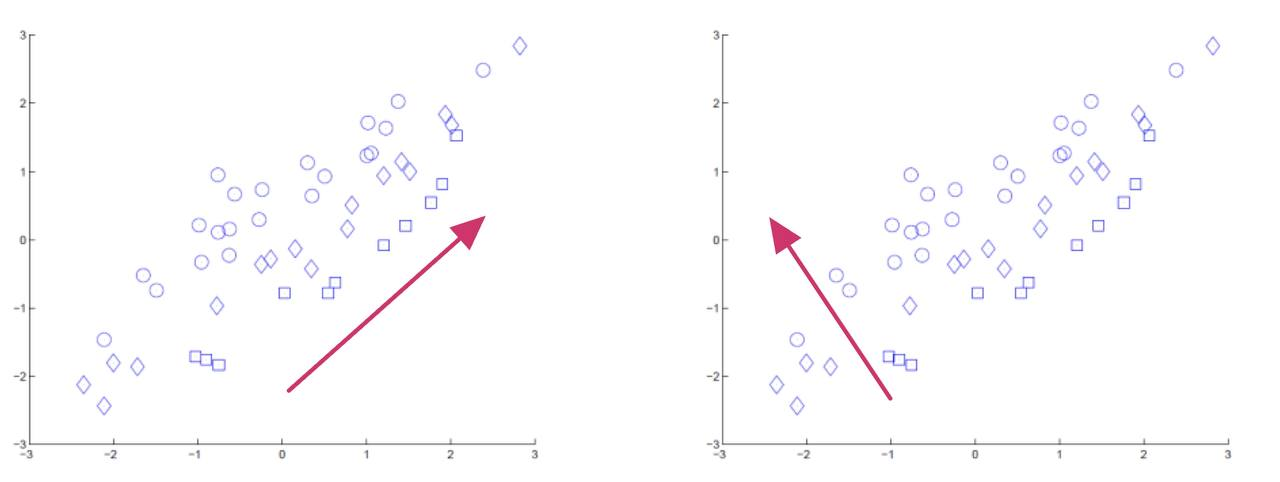
\includegraphics[width=0.9\textwidth]{"image/Q3_a.jpg"}
        \end{figure}
        \item [(b)] CCA
        \begin{figure}[H]
            \centering
            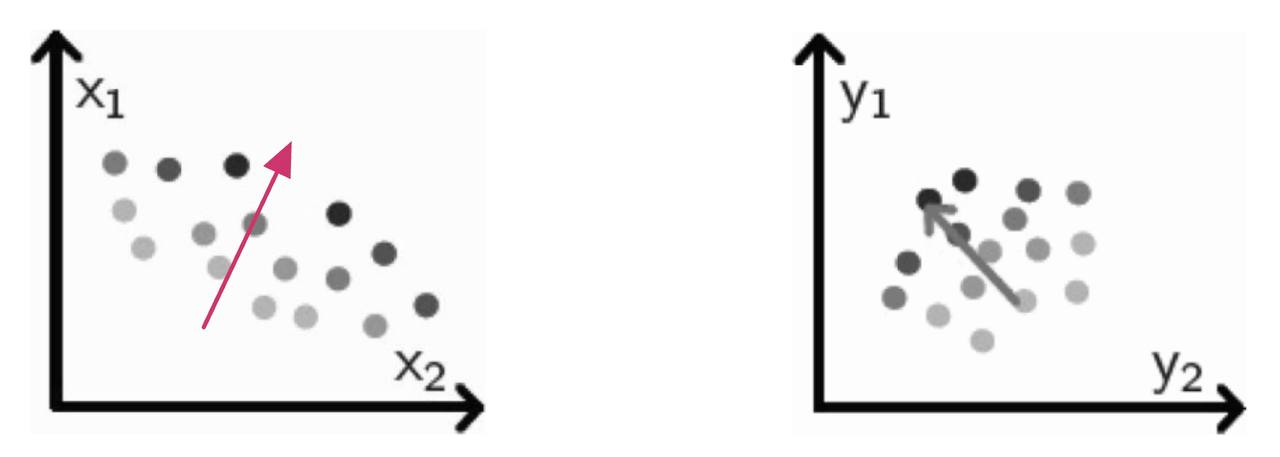
\includegraphics[width=0.9\textwidth]{"image/Q3_b.jpg"}
        \end{figure}
        \item [(c)] PCA\newline
        {\bf Solution:}
        \par Let $\b{x}=\begin{bmatrix}
            x_1\\
            x_2
        \end{bmatrix}$ and $\b{\mu}=\E[\b{x}]=\begin{bmatrix}
            \E[x_1]\\\E[x_2]
        \end{bmatrix}=\begin{bmatrix}
            0\\0
        \end{bmatrix}$, then $\Sigma=\E[(\b{x}-\b{\mu})(\b{x}-\b{\mu})^T]=\E[\b{x}\b{x}^T]=\begin{bmatrix}
            \E[x_1^2] & \E[x_1x_2]\\
            \E[x_1x_2] & \E[x_2^2]
        \end{bmatrix} = \begin{bmatrix}
            \frac{2}{3} & \frac{2}{3}\\
            \frac{2}{3} & \frac{2}{3}
        \end{bmatrix}$.
        \par By solving eigen value, we have two eigen values of $\Sigma$, $\lambda_1 = \frac{4}{3}$ and $\lambda_2=0$, we choose the eigen corresponding to $\lambda_1$ as first principal component, which is $\b{u}=\begin{bmatrix}
            1\\1
        \end{bmatrix}\Rightarrow\b{w}=\begin{bmatrix}
            \frac{\sqrt{2}}{2}\\\frac{\sqrt{2}}{2}
        \end{bmatrix}$.
        \par Then the projected coordinates of data are $(-1,-1)\to -\sqrt{2}$, $(0,0)\to 0$ and $(1,1)\to \sqrt{2}$. Then variance of projected data is $\frac{4}{3}$

    \end{enumerate}
    \item [4.][Dimension Reduction]
    \begin{enumerate}
        \item [(a)] PCA
        {\bf Proof:}
        \par The optimization problem is as following
        \begin{maxi}|l|
            {\b{w}_1}{\b{w}_1^T\b{\Sigma}\b{w}_1}{}{}
            \addConstraint{||\b{w}_1||=1}{}
        \end{maxi}
        Then the Lagrangian fucntion is 
        \[\mathcal{L}(\b{w}_1,\alpha)=-\b{w}_1^T\b{\Sigma}\b{w}_1+\alpha(\b{w}_1^T\b{w}_1-1)\]
        then
        \begin{align*}
            \PARTIAL{\mathcal{L}}{\b{w}_1}=-2\b{\Sigma}\b{w}_1+2\alpha\b{w}_1=0\Rightarrow\b{\Sigma}\b{w}_1^\star=\alpha^\star\b{w}_1^\star
        \end{align*}
        and 
        \begin{align*}
            (\b{w}_1^\star)^T\b{\Sigma}\b{w}_1^\star = \alpha^\star(\b{w}_1^\star)^T\b{w}_1^\star=\alpha^\star
        \end{align*}
        In order to maximize $\b{w}_1^T\b{\Sigma}\b{w}_1$, we need to choose the maximum eigen value $\alpha$ of $\b{\Sigma}$. Thus, $\b{w}_1$ is the principal component.
        \item [(b)] PCA vs LDA
        {\bf Solution:}
        \par LDA is a method that aims to find a projection direction such that the projected data have the maximum distances between classes and minimum variance within classes.
        \begin{enumerate}
            \item [1.] Similarity
            \par Both of LDA and PCA solve the same class of optimization problem (Generalized Rayleigh quotient or eigenvalue problem).
            \item [2.] Difference
            \par PCA is an un-supervised method while LDA is a supervised method. Moreover, PCA aims to maximize the variance of projected data but LDA aims to maximize the distance between difference classes and minimize the variance of each classes at the same time.
        \end{enumerate}
        \item [(c)] show that $\b{w_1}$ minimizes the reconstruction error $||\b{X-Xwx}^T||^2_F$ for any $\b{w}$ satifisying $||\b{w}||_2=1$.\newline
        {\bf Proof:}
        \par In order to minimize reconstruction error, we need to rewrite the reconstruction error
        \begin{align*}
            ||\b{X}-\b{Xww}^T||^2_F&=\sum_{i=1}^N||\b{x}_i-\b{ww}^T\b{x}_i||^2\\
            &=\sum_{i=1}^N (\b{x}_i-\b{ww}^T\b{x}_i)^T(\b{x}_i-\b{ww}^T\b{x}_i)\\
            &=\sum_{i=1}^N \b{x_i}^T\b{x}_i-2\b{x}_i^T\b{ww}^T\b{x}_i+\b{x}_i^T\b{ww}^T\b{ww}^T\b{x}_i\\
            &=\sum_{i=1}^N \b{x_i}^T\b{x}_i-2(\b{w}^T\b{x}_i)^2+||\b{w}||_2^2(\b{w}^T\b{x}_i)^2
        \end{align*}
        Given that $||\b{w}||_2^2=1$, we have 
        \begin{align*}
            ||\b{X}-\b{Xww}^T||^2_F&=\sum_{i=1}^N \b{x_i}^T\b{x}_i-(\b{w}^T\b{x}_i)^2
        \end{align*}
        Thus, minimizing reconstruction error is equivalent to maximizing $\sum_{i=1}^N (\b{w}^T\b{x}_i)^2$. Moreover, since $\b{X}$ is a cnetered sample matrix, we know that $\E[\b{x}_i]=0$. Therefore, we have 
        \begin{align*}
            \E[\b{w}^T\b{x}_i]&=0\\
            \Var(\b{w}^T\b{x}_i)&=\E[(\b{w}^T\b{x}_i)^2]-\E[\b{w}^T\b{x}_i]\\
            &=\E[(\b{w}^T\b{x}_i)^2]\\
            &=\frac{1}{N} \sum_{i=1}^N (\b{w}^T\b{x}_i)^2
        \end{align*}
        Thus, we know that maximizing $\sum_{i=1}^N (\b{w}^T\b{x}_i)^2$ is equivalent to maximizing $\Var(\b{w}^T\b{x}_i)$, which is exactly same to PCA problem, so their solutions are consistent.
    \end{enumerate}

    
\end{enumerate}
\includepdfmerge{HW3-Coding.pdf,1-5}
\end{document}